\documentclass[]{spie}
\renewcommand{\baselinestretch}{1.0}

\usepackage{algorithm}
\usepackage{algpseudocode}
\usepackage{pgf}
\usepackage{tikz}
\usetikzlibrary{intersections}
\usetikzlibrary{arrows.meta,calc,positioning,fit,shapes.misc}
\usetikzlibrary{backgrounds,shapes.geometric,math}
\usepackage{pgfplots}
\usepackage{amsmath,amsfonts,amssymb}
\usepackage{graphicx}
\usepackage{booktabs}
\usepackage[colorlinks=true, allcolors=blue]{hyperref}

\title{Bayesian Network Guided Vulnerability Analysis of Detection, Fusion Continuity, and Sensor Handoffs for Aircraft Custody in Terminal Airspace}

\author[a]{Amir K. Saeed}
\author[a]{Alhassan S. Yasin, PhD}
\author[a]{Benjamin A. Johnson}
\author[a]{Omar Ramadan}
\author[a]{Benjamin M. Rodriguez, PhD}
\affil[a]{Whiting School of Engineering EP Program, Johns Hopkins University}

\authorinfo{Further author information: Send correspondence to asaeed7@jhu.edu}

\pagestyle{empty}
\setcounter{page}{301}

\begin{document}
\maketitle

% ======================================================================
% ABSTRACT
% ======================================================================
\begin{abstract}
Persistent custody of aircraft in terminal airspace depends on a chain of interdependent conditions, satellite availability, sensor detection, inter-satellite handoffs, precision tracking, fusion continuity, and identity persistence. Identifying which links in this chain are most vulnerable to failure is a prerequisite for principled system design. Building on the GoDSAT reinforcement learning framework and the Design of Experiments–Bayesian Network (DoE-BN) methodology established in prior work, this paper constructs a seven-node BN over the GoDSAT custody chain and applies do-calculus interventions to rank failure modes and quantify mitigations. A Python reimplementation of the GoDSAT 16-satellite CONUS constellation enables 270 simulation runs across three sensor modalities (ADS-B, Mode-S, MLAT) under a full-factorial DoE. The baseline custody rate is 0.705 (95\% CI [0.697, 0.712]). BN vulnerability analysis identifies fusion continuity as the dominant failure mode ($\Delta = +0.985$), not detection as in prior kill chain studies. Perfect availability yields the largest mitigation gain (+34.5\%), while hysteresis reduces custody by 13.9\% by blocking timely handoffs. DoE Random Forest analysis assigns 99.9\% of custody variance to sensor type: Mode-S at a 4-second update interval is structurally incompatible with a 2-second tracking loop, producing zero custody regardless of constellation size or target count. These results establish sensor update rate as an architectural constraint and provide a reproducible BN-guided framework for terminal airspace custody vulnerability assessment.
\end{abstract}

\keywords{Bayesian networks, multi-sensor fusion, aircraft custody, sensor handoffs, vulnerability analysis, evaluation, verification and validation, risk reduction}

% ======================================================================
% 1. INTRODUCTION
% ======================================================================
\section{INTRODUCTION}
\label{sec:intro}

Persistent custody of aircraft in terminal airspace is a critical requirement for safe and efficient air traffic management. Terminal airspace, the high-density region surrounding major airports, presents unique challenges: multiple aircraft arriving and departing simultaneously, diverse sensor modalities with different update rates and coverage geometries, and handoff events that must occur seamlessly as aircraft transition between sensor fields of view. Custody loss, defined as the failure to maintain continuous, identity-aware tracking of an aircraft, can lead to dangerous gaps in situational awareness. Understanding which phases of the custody chain are most vulnerable to failure is therefore essential for system designers and operators.

The GoDSAT framework~\cite{Saeed2026GoDSATRL} introduced reinforcement learning (RL)-enabled custody transfer for satellite constellations, demonstrating persistent coverage through a proximity-based ClaimMap and pretrained Q-tables. GoDSAT validated custody through dwell time, handoff latency, and policy reusability metrics, confirming that RL-enabled transfer is a viable foundation for scalable autonomous tasking. However, GoDSAT does not quantify which phases of the custody chain are most vulnerable to failure, nor does it evaluate how sensor architecture choices, particularly sensor update rate relative to the tracking loop, affect system-level custody probability. Identifying these vulnerabilities is a prerequisite for principled mitigation design.

Saeed et al.~\cite{Saeed2025DOEFramework} established a systematic framework combining Design of Experiments (DoE) with Bayesian Network (BN) modeling for defense system vulnerability analysis, demonstrating the approach on the kill chain from Ball's one-on-one engagement model~\cite{Ball2003}. That work found that aircraft altitude dominates detection probability, while~\cite{Saeed2025BNDOE} extended the methodology by introducing surrogate modeling to bridge disparate simulation environments through BN inference. Together, these works established DoE-BN as a rigorous, data-driven path to vulnerability ranking in defense simulations. This paper applies that methodology to a fundamentally different problem: not the kill chain from threat to aircraft destruction, but the custody chain from sensor availability through fusion continuity to maintained tracking.

This work makes three contributions. First, we develop a Python reimplementation of the GoDSAT constellation~\cite{Saeed2026GoDSATRL} that enables headless Monte Carlo execution across three sensor modalities; ADS-B~\cite{adsb_faa}, Mode-S, and MLAT~\cite{opensky}. Second, we construct a seven-node BN over the custody chain and apply do-calculus interventions~\cite{Koller2009} to rank failure modes and quantify mitigations. Third, we conduct a full-factorial DoE over operational factors following Saeed et al.~\cite{Saeed2025DOEFramework}, using Random Forest importance~\cite{Breiman2001} to identify sensor type as the dominant architectural driver of custody probability. Section~\ref{sec:background} reviews related work. Section~\ref{sec:methodology} describes the simulation, BN construction, and DoE design. Section~\ref{sec:analysis} presents results. Section~\ref{sec:conclusion} concludes.

% ======================================================================
% 2. RELATED WORK AND BACKGROUND
% ======================================================================
\section{Related Work and Background}
\label{sec:background}

This section establishes the two bodies of prior work that this paper synthesizes. Section~\ref{sec:bn_background} reviews Bayesian Network methodology for defense vulnerability analysis, tracing the lineage from Ball's one-on-one engagement model \cite{Ball2003} through the DoE-BN framework of \cite{Saeed2025DOEFramework,Saeed2025BNDOE} that this paper extends. Section~\ref{sec:godsat_background} describes the GoDSAT framework \cite{Saeed2026GoDSATRL} that provides the simulation environment and custody chain definition on which the BN is constructed. Together these two threads motivate the core 
contribution: applying a validated probabilistic vulnerability methodology to a new domain, custody continuity in terminal airspace, where the dominant failure mode and mitigation structure differ qualitatively from the kill chain analyses in prior work.

\subsection{Bayesian Networks for Defense Vulnerability Analysis}
\label{sec:bn_background}

Bayesian Networks are probabilistic graphical models in which nodes represent random variables and directed edges encode conditional dependencies~\cite{Pearl1988}. The joint distribution over all nodes factorizes as the product of each node's conditional distribution given its parents, enabling efficient exact inference over complex dependency structures~\cite{Koller2009}. In defense applications, BNs are particularly valuable because they support both forward inference, predicting system-level outcomes from component probabilities, and diagnostic inference, identifying which upstream failure most explains an observed custody loss. This bidirectional reasoning is essential for operational vulnerability analysis where the causal structure of the system is known but the relative importance of failure modes is not. Figure~\ref{fig:tikz_tree} reproduces the one-on-one engagement tree from Ball~\cite{Ball2003}, as used in the DoE-BN kill chain analysis of \cite{Saeed2025DOEFramework,Saeed2025BNDOE}. Each branch represents a conditional probability event; the aircraft is killed only if all six phases succeed sequentially.

\begin{figure}[h]
\begin{center}
    \begin{tikzpicture}[
        level distance=2cm,
        sibling distance=1.5cm,
        edge from parent/.style={draw, thick, -latex}
    ]

    % Upper Left Image
    \node[anchor=south west] at (-5, -1) {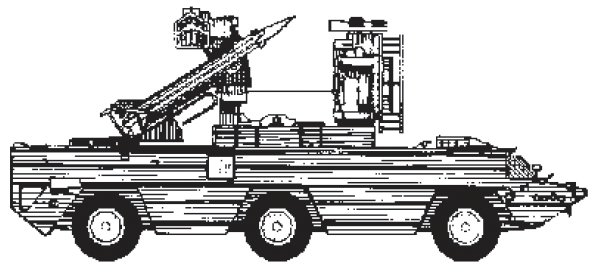
\includegraphics[width=2cm]{figures/weapon.png}};
    
    % Upper Right Image
    \node[anchor=south east] at (7, -1) {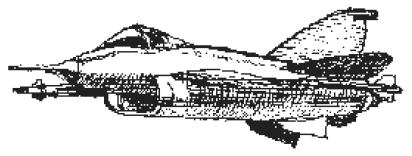
\includegraphics[width=2cm]{figures/aircraft.png}};
    
    \node {(0)}
        child {node{} 
        edge from parent node[left] { $P^c_A$ }
        edge from parent node[midway, shift={(1.3,0.0)}] {$P_A$}}
        child {node{(1)}
            child {node{} 
            edge from parent node[left] { $P^c_{D|A}$}
            edge from parent node[midway, shift={(1.3,0.0)}] {$P_{D|A}$}}
            child {node{(2)}
                child {node{}
                edge from parent node[left] { $P^c_{L|D}$}
                edge from parent node[midway, shift={(1.3,0.0)}] {$P_{L|D}$}}
                child {node{(3)}
                    child {node{}
                    edge from parent node[left] { $P^c_{I|L}$}
                    edge from parent node[midway, shift={(1.3,0.0)}] {$P_{I|L}$}}
                    child {node{(4)}
                        child {node{}
                        edge from parent node[left] { $P^c_{H|I}$}
                        edge from parent node[midway, shift={(1.3,0.0)}] {$P_{H|I}$}}
                        child {node{(5)}
                            child {node{$P_S$}
                            edge from parent node[left] { $P^c_{K|H}$}
                            edge from parent node[midway, shift={(1.3,0.0)}] {$P_{K|H}$}}
                            child {node{$P_K$}
                            }
                        }
                    }
                }
            }
        };

    % Additional Text Inside tikzpicture
    \node at (2,-12.5) {where $P_S = P^c_K = 1 - P_K$ (The aircraft survives the scenario.) and};
    \node at (3.45,-13) {$P_K = P_A P_{D|A} P_{L|D} P_{I|L} P_{H|I} P_{K|H}$ (The aircraft is killed in the scenario.)};  

    % Vertical Pulse Signal 1
    \draw[thick, -latex] 
        (-6.5,0) -- (-6.5,-0.7)  % Flat Line
        -- (-6.5,-0.8)         % Small Rise
        -- (-6.2,-0.9)        % Sharp Drop
        -- (-6.7,-1.0)         % Sharp Peak
        -- (-6.5,-1.1)       % Back to Baseline
        -- (-6.5,-1.9);
    % Vertical Pulse Signal 2
    \draw[thick, -latex] 
        (-6.5,-1.9) -- (-6.5,-2.6)  % Flat Line
        -- (-6.5,-2.7)         % Small Rise
        -- (-6.2,-2.8)        % Sharp Drop
        -- (-6.7,-2.9)         % Sharp Peak
        -- (-6.5,-3.0)         % Back to Baseline
        -- (-6.5,-3.9);
    % Vertical Pulse Signal 3
    \draw[thick, -latex] 
        (-6.5,-3.9) -- (-6.5,-4.5)  % Flat Line
        -- (-6.5,-4.6)         % Small Rise
        -- (-6.2,-4.7)        % Sharp Drop
        -- (-6.7,-4.8)         % Sharp Peak
        -- (-6.5,-4.9)         % Back to Baseline
        -- (-6.5,-5.8);
     % Vertical Pulse Signal 4
    \draw[thick, -latex] 
        (-6.5,-5.8) -- (-6.5,-6.6)  % Flat Line
        node[midway, shift={(-0.25,0.0)}, rotate=90] {Time}
        -- (-6.5,-6.7)         % Small Rise
        -- (-6.2,-6.8)        % Sharp Drop
        -- (-6.7,-6.9)         % Sharp Peak
        -- (-6.5,-7.0)         % Back to Baseline
        -- (-6.5,-7.9);    
    % Vertical Pulse Signal 5
    \draw[thick, -latex] 
        (-6.5,-7.9) -- (-6.5,-8.5)  % Flat Line
        -- (-6.5,-8.6)         % Small Rise
        -- (-6.2,-8.7)        % Sharp Drop
        -- (-6.7,-8.8)         % Sharp Peak
        -- (-6.5,-8.9)         % Back to Baseline
        -- (-6.5,-9.8);  
    % Vertical Pulse Signal 6
    \draw[thick, -latex] 
        (-6.5,-9.8) -- (-6.5,-10.4)  % Flat Line
        -- (-6.5,-10.5)         % Small Rise
        -- (-6.2,-10.6)        % Sharp Drop
        -- (-6.7,-10.7)         % Sharp Peak
        -- (-6.5,-10.8)         % Back to Baseline
        -- (-6.5,-11.7); 

    % Time Labels
    \node[right] at (-6.2,-2.0) {The exposure part of the};
    \node[right] at (-6.2,-2.35) {scenario begins when the};
    \node[right] at (-6.2,-2.6) {aircraft enters into the air};
    \node[right] at (-6.2,-2.95) {space defended by an active};
    \node[right] at (-6.2,-3.2) {threat.};

    \node[right] at (-6.2,-4.7) {The encounter begins when};
    \node[right] at (-6.2,-5.05) {the aircraft is detected.};

    \node[right] at (-6.2,-6.6) {The engagement begins};
    \node[right] at (-6.2,-6.95) {when a gun is fired or a };
    \node[right] at (-6.2,-7.3) {missile is launched.};

    \node[right] at (-6.2,-8.5) {The endgame begins};
    \node[right] at (-6.2,-8.85) {when the propagator};
    \node[right] at (-6.2,-9.2) {intercepts the aircraft.};

    \node[right] at (-6.2,-10.2) {The vulnerability phase};
    \node[right] at (-6.2,-10.55) {of the endgame begins when};
    \node[right] at (-6.2,-10.9) {the aircraft is hit by the warhead};
    \node[right] at (-6.2,-11.25) {on the propagator};

    \draw[thick, <->, latex-latex] (8,0) -- (8,-5.8) 
        node[midway, shift={(-0.25,0.0)}, rotate=90] {$P_{SS}$}; % Right Arrow with Rotated Text
    \draw[thick, <->, latex-latex] (8,-5.8) -- (8,-11.7) 
        node[midway, shift={(-0.25,0.0)}, rotate=90] {$P_{K|SS}$}; % Right Arrow with Rotated Text

    \draw[thick, <->, latex-latex] (8.3,0) -- (8.3,-9.8) 
        node[midway, shift={(0.25,0.0)}, rotate=-90] {Susceptibility, $P_{H}$}; % Right Arrow with Rotated Text
    \draw[thick, <->, latex-latex] (8.3,-9.8) -- (8.3,-11.7) 
        node[midway, shift={(0.25,0.0)}, rotate=-90] {Vulnerability, $P_{K|H}$}; % Right Arrow with Rotated Text

    \node[right] at (1.3,-0.8) {The active weapon};
    \node[right] at (1.5,-1.15) {searches for aircraft.};

    \node[right] at (2.0,-2.8) {The weapon's target detection};
    \node[right] at (2.2,-3.15) {sensors detect an aircraft.};

    \node[right] at (2.7,-4.6) {The detected aircraft is tracked,};
    \node[right] at (2.9,-4.95) {a fire control solution is};
    \node[right] at (3.1,-5.3) {obtained, and a propagator};
    \node[right] at (3.3,-5.65) {is launched.};

    \node[right] at (3.5,-6.8) {The propagator 'flies' out};
    \node[right] at (3.7,-7.15) {towards an intercept with};
    \node[right] at (3.9,-7.5) {the aircraft.};

    \node[right] at (4.3,-8.9) {The propagator};
    \node[right] at (4.5,-9.25) {hits the aircraft.};

    \node[right] at (5.0,-10.7) {The aircraft};
    \node[right] at (5.2,-11.05) {killed by the};
    \node[right] at (5.4,-11.4) {propagator hit.};

    \end{tikzpicture}
\end{center}
    \caption{Tree diagram for the one-on-one scenario (single shot) - Original figure from Ball (2003)~\cite{Ball2003}.}
    \label{fig:tikz_tree}
\end{figure}

Ball~\cite{Ball2003} formalized the one-on-one engagement as a sequential BN over six phases: weapon activation, detection, launch, intercept, hit, and kill. Each phase is conditioned on the previous, and the overall kill probability is the product of all conditional probabilities along the chain. Saeed et al.~\cite{Saeed2025DOEFramework} applied DoE to systematically explore factor interactions affecting detection probability in this kill chain model, combining Random Forest classification with ANOVA to identify aircraft altitude as the dominant factor.~\cite{Saeed2025BNDOE} extended this by training surrogate models on simulation outputs to estimate conditional probabilities for each BN node, enabling rapid exploration of the trade space without re-running expensive simulations. This paper adapts the same DoE-BN methodology to a structurally similar but operationally distinct problem: the custody chain in terminal airspace surveillance.

The custody chain differs from the kill chain in two important ways. First, custody is a continuous maintenance problem rather than a discrete engagement event, the system must sustain tracking across time, sensor handoffs, and coverage gaps rather than executing a single sequential engagement. Second, the dominant failure mode is not detection probability but fusion continuity: the ability to maintain a sufficient consecutive sequence of confirmed detections to sustain precision tracking. As shown in Section~\ref{sec:analysis}, this structural difference produces a qualitatively different vulnerability ranking than the one reported for the kill chain in~\cite{Saeed2025DOEFramework}.

\subsection{The GoDSAT Framework and Custody Transfer}
\label{sec:godsat_background}

GoDSAT~\cite{Saeed2026GoDSATRL} is a MATLAB simulation framework for RL-enabled custody transfer in satellite constellations. The framework integrates Keplerian orbit propagation, ballistic target trajectories, and a global ClaimMap that enforces exclusive target ownership across the constellation. At each simulation timestep, ownership of a target is assigned to the satellite with minimum Euclidean distance in ECEF coordinates, and a pretrained Q-table policy executes one-bin azimuth-elevation hill-climb steps to maintain target centering within the field of view. The 16-satellite, two-plane constellation (RAAN $50^\circ$ and $120^\circ$, $a = 2000$~km, $e = 0.1$, $i = 90^\circ$, $dt = 2$~s) demonstrated persistent coverage of 20 ballistic targets over CONUS with high custody duration and low handoff latency. This paper uses the GoDSAT constellation as its simulation baseline and maps GoDSAT's internal signals to BN node observables.

The BN nodes constructed in this paper correspond directly to GoDSAT signals. Availability ($A$) is true when a satellite is live and has detected the target in the current tick. Detection ($D$) is true when the target falls within the satellite's field-of-view cone. Handoff ($H$) is true when the ClaimMap ownership assignment changes between ticks, corresponding to the custody transfer event formalized in Algorithm~1 of~\cite{Saeed2026GoDSATRL}. Precision tracking ($Q$) is true when at least three consecutive detections have been observed, mirroring GoDSAT's Q-mode entry condition. Fusion continuity ($F$) is true when $Q$ has been sustained for at least three consecutive ticks. Identity persistence ($I$) is true when the target has been continuously tracked for at least ten seconds. Custody ($C$) is defined as the conjunction $A \wedge Q \wedge F$, reflecting the requirement for simultaneous availability, precision tracking, and sustained fusion continuity. The resulting seven-node custody BN, with directed edges and marginal probabilities $P(\cdot)$ estimated from 
baseline Monte Carlo runs, is shown in Figure~\ref{fig:bn_structure}.

% ======================================================================
% 3. METHODOLOGY
% ======================================================================
\section{Methodology}
\label{sec:methodology}

This section describes the three-component methodology used to produce the vulnerability 
analysis. Section~\ref{sec:sim} details the Python simulation framework that reimplements 
the GoDSAT constellation~\cite{Saeed2026GoDSATRL} across three sensor modalities and executes Monte Carlo runs to generate BN signal data. Section~\ref{sec:bn} describes the seven-node BN construction, CPT estimation from simulation output, and the do-calculus intervention framework used to rank failure modes and quantify mitigations. Section~\ref{sec:doe} presents the full-factorial Design of Experiments over four operational factors, following the methodology of \cite{Saeed2025DOEFramework}, and the Random Forest importance analysis used to identify the dominant architectural driver of custody probability. Together these three components form a reproducible pipeline from orbital simulation to probabilistic vulnerability assessment.

\subsection{Python Simulation Framework}
\label{sec:sim}

The simulation reimplements the GoDSAT constellation~\cite{Saeed2026GoDSATRL} in Python to enable headless Monte Carlo execution without MATLAB licensing constraints. The constellation consists of 16 satellites in two orbital planes with RAAN values of $50^\circ$ and $120^\circ$, semi-major axis $a = 2000$~km, eccentricity $e = 0.1$, inclination $i = 90^\circ$, and argument of perigee $\omega = 270^\circ$. Mean anomalies are staggered at $45^\circ$ intervals to phase satellites evenly within each plane. Keplerian propagation follows the formulation of~\cite{Saeed2026GoDSATRL}: the mean anomaly evolves as $M(t) = M_0 + nt$ where $n = \sqrt{\mu/a^3}$, and Kepler's equation is solved by Newton--Raphson iteration to obtain true anomaly. Positions are transformed from perifocal to ECI and then to ECEF coordinates. A target is considered visible if the angular separation between satellite and target boresight does not exceed the half-cone field-of-view angle. Twenty aircraft targets follow great-circle trajectories across CONUS, and the simulation runs for 7200~seconds at $dt = 2$~s per tick.

Satellite positions are propagated from classical orbital elements using Keplerian mechanics. The mean anomaly evolves as:

\begin{equation}
    M(t) = M_0 + n t, \qquad n = \sqrt{\frac{\mu}{a^3}}
    \label{eq:mean_anomaly}
\end{equation}

where $\mu = 3.986 \times 10^{14}$~m$^3$s$^{-2}$ is Earth's gravitational parameter. Kepler's equation $M = E - e\sin E$ is solved for eccentric anomaly $E$ by Newton--Raphson iteration, and true anomaly $\nu$ is recovered via:

\begin{equation}
    \tan\frac{\nu}{2} = \sqrt{\frac{1+e}{1-e}}
    \tan\frac{E}{2}
    \label{eq:true_anomaly}
\end{equation}

The satellite position vector in ECEF coordinates is obtained by the rotation sequence:

\begin{equation}
    \mathbf{r}_{\mathrm{ECEF}}(t) = 
    R_z(\omega_E t)\, R_3(-\Omega)\, R_1(-i)\, 
    R_3(-\omega)\, \mathbf{r}_{\mathrm{PQW}}(t)
    \label{eq:ecef}
\end{equation}

where $\omega_E = 2\pi/86164.09$~rad/s is Earth's rotation rate, $\Omega$ is the right ascension of the ascending node, $i$ is inclination, $\omega$ is argument of perigee, and $\mathbf{r}_{\mathrm{PQW}}$ is the position in the perifocal frame. A target $T_i$ is visible to satellite $S_j$ when the line-of-sight (LOS) condition is satisfied:

\begin{equation}
    \mathrm{LOS}(S_j, T_i) = 
    \begin{cases}
        1 & \text{if } \arccos\!\left(
        \dfrac{\hat{\mathbf{r}}_{S_j}(t) \cdot 
            \hat{\mathbf{r}}_{T_i}(t)}
        {\|\mathbf{r}_{S_j}(t)\|\, 
        \|\mathbf{r}_{T_i}(t)\|}
        \right) \leq \theta_{\mathrm{FOV}} \\[6pt]
        0 & \text{otherwise}
    \end{cases}
    \label{eq:los}
    \end{equation}
    
where $\theta_{\mathrm{FOV}}$ is the sensor half-cone angle. At each tick, a detection 
is recorded with probability $p_{\mathrm{det}}$ conditioned on LOS:

\begin{equation}
    d_{j,i}(t) \sim 
    \mathrm{Bernoulli}(p_{\mathrm{det}} \cdot 
    \mathrm{LOS}(S_j, T_i, t))
    \label{eq:detection}
\end{equation}

Three sensor modalities are modeled, each with distinct update intervals and detection probabilities. ADS-B~\cite{adsb_faa} updates at 1~Hz with detection probability $p_{\mathrm{det}} = 0.99$, consistent with FAA equipage requirements for controlled airspace. Mode-S interrogation updates every 4~seconds with $p_{\mathrm{det}} = 0.95$, reflecting the standard secondary surveillance radar reply cadence. Multilateration (MLAT)~\cite{opensky} updates every 2~seconds with $p_{\mathrm{det}} = 0.90$, consistent with reported OpenSky network performance. At each tick, a Bernoulli draw against $p_{\mathrm{det}}$ determines whether a detection is recorded for each visible target--satellite pair. The BN signal for each tick is derived from these detection outcomes according to the node definitions in Section~\ref{sec:background}.

\subsection{Bayesian Network Construction and CPT Estimation}
\label{sec:bn}

The custody BN is a directed acyclic graph (DAG)~\cite{Pearl1988} over seven binary nodes: $\{A, D, H, Q, F, I, C\}$. The topology encodes the causal structure of the custody chain: $D$ depends on $A$; $Q$ depends on $D$ and $H$; $F$ depends on $Q$; $I$ depends on $D$ and $H$; and $C$ depends on $A$, $Q$, and $F$. The joint distribution factorizes as:

\begin{equation}
    P(A,D,H,Q,F,I,C) = P(A)\,P(D \mid A)\,P(H)\,P(Q \mid D,H)\,P(F \mid Q)\,P(I \mid D,H)\,P(C \mid A,Q,F)  
    \label{eq:joint}
\end{equation}

Conditional probability tables (CPTs) are estimated directly from simulation output 
using Laplace smoothing with pseudocount $\alpha = 1$ to avoid zero-probability cells. 
For a node $X$ with parent configuration $\mathbf{pa}$:

\begin{equation}
    \hat{P}(X{=}1 \mid \mathbf{pa}) = 
    \frac{n_{1|\mathbf{pa}} + \alpha}
        {n_{\mathbf{pa}} + 2\alpha}
    \label{eq:laplace}
\end{equation}

where $n_{1|\mathbf{pa}}$ is the count of $X{=}1$ observations given $\mathbf{pa}$, 
and $n_{\mathbf{pa}}$ is the total count for that parent configuration. 

Table~\ref{tab:cpt} reports representative 
estimated CPT values for selected parent 
configurations from the baseline Monte Carlo 
run, illustrating the strength of conditional 
dependencies in the custody chain.

\begin{table}[h]
\caption{Representative estimated CPT values 
from baseline Monte Carlo (ADS-B, 50 runs). 
Laplace smoothing with $\alpha = 1$ applied.}
\label{tab:cpt}
\centering
\begin{tabular}{llc}
\toprule
Node & Parent configuration & 
$\hat{P}(X{=}1 \mid \mathbf{pa})$ \\
\midrule
$D$ & $A{=}1$ & 0.99 \\
$D$ & $A{=}0$ & 0.01 \\
$Q$ & $D{=}1,\, H{=}0$ & 0.94 \\
$Q$ & $D{=}1,\, H{=}1$ & 0.41 \\
$Q$ & $D{=}0,\, H{=}0$ & 0.02 \\
$F$ & $Q{=}1$ & 0.97 \\
$F$ & $Q{=}0$ & 0.01 \\
$C$ & $A{=}1,\, Q{=}1,\, F{=}1$ & 0.99 \\
$C$ & $A{=}1,\, Q{=}1,\, F{=}0$ & 0.01 \\
$C$ & $A{=}0,\, Q{=}1,\, F{=}1$ & 0.01 \\
\bottomrule
\end{tabular}
\end{table}

The CPT values reveal two important structural properties of the custody chain. First, the handoff effect on precision tracking is substantial: $\hat{P}(Q{=}1 \mid D{=}1, H{=}1) = 0.41$ versus $\hat{P}(Q{=}1 \mid D{=}1, H{=}0) = 0.94$, confirming that ownership transfers temporarily disrupt the consecutive detection counter required for $Q$-mode entry, even though handoffs ultimately enable custody by passing ownership to better-positioned satellites. Second, fusion continuity is highly robust once precision tracking is established: $\hat{P}(F{=}1 \mid Q{=}1) = 0.97$, meaning that the primary challenge is achieving and sustaining $Q$, not converting $Q$ into $F$.

Exact forward inference marginalizes over all $2^7 = 128$ joint configurations:

\begin{equation}
    P(C{=}1) = \sum_{\mathbf{x} \,:\, x_C = 1}
    P(A{=}x_A)\, P(D{\mid}A)\, P(H)\, 
    P(Q{\mid}D,H)\, P(F{\mid}Q)\, 
    P(I{\mid}D,H)\, P(C{\mid}A,Q,F)
    \label{eq:inference}
\end{equation}

Vulnerability analysis applies Pearl's do-calculus intervention~\cite{Koller2009}. 
For each upstream node $X_i$, the vulnerability delta is:

\begin{equation}
    \Delta_i = P(C{=}1) - 
    P\!\left(C{=}1 \mid \mathrm{do}(X_i{=}0)\right)
    \label{eq:delta}
\end{equation}

where $\mathrm{do}(X_i{=}0)$ forces node $X_i$ to fail by setting its CPT column to 
zero, severing all incoming edges. Mitigation analysis applies the complementary 
intervention:

\begin{equation}
    \Gamma_i = P\!\left(C{=}1 \mid 
    \mathrm{do}(X_i{=}1)\right) - P(C{=}1)
    \label{eq:mitigation}
\end{equation}

A large positive $\Delta_i$ identifies $X_i$ as a high-vulnerability node; a large 
positive $\Gamma_i$ identifies $X_i$ as a high-value mitigation target.

\subsection{Design of Experiments Factor Analysis}
\label{sec:doe}

Following the DoE methodology of~\cite{Saeed2025DOEFramework}, a full-factorial design was constructed over four operational factors: sensor type $\in \{\mathrm{ADS\text{-}B},\, \mathrm{Mode\text{-}S},\, \mathrm{MLAT}\}$, number of satellites $\in \{8, 12, 16\}$, number of targets $\in \{10, 20, 30\}$, and simulation duration $\in \{3600\,\mathrm{s},\, 7200\,\mathrm{s}\}$. The factor ranges bracket the GoDSAT baseline configuration~\cite{Saeed2026GoDSATRL}, 16 satellites, 20 targets, and 7200~s, ensuring that the baseline lies within the interior of the factor space rather than at its boundary. The full factorial yields $3 \times 3 \times 3 \times 2 = 54$ unique configurations. Each configuration was replicated across five independent random seeds, producing $54 \times 5 = 270$ simulation runs in total.

For each of the 270 runs, the mean custody rate, standard deviation, mean detection rate, and mean handoff count were recorded. Main effects were computed as the deviation of each factor level's mean custody from the grand mean across all runs. Feature importance was estimated using a Random Forest regressor~\cite{Breiman2001} trained on the 54 per-configuration mean custody rates with the four factors as predictors, following the Gini impurity importance methodology used in~\cite{Saeed2025DOEFramework}. The Random Forest was trained with 200 estimators, and importance scores were normalized to sum to unity.

The full-factorial design generates 
$N = \prod_{k=1}^{K} L_k$ configurations, 
where $K = 4$ factors have $L_k$ levels each:
\begin{equation}
    N = L_{\mathrm{sensor}} \times 
    L_{\mathrm{sats}} \times 
    L_{\mathrm{targets}} \times 
    L_{\mathrm{duration}} = 
    3 \times 3 \times 3 \times 2 = 54
    \label{eq:factorial}
\end{equation}

The main effect for factor $k$ at level $\ell$ 
is the deviation from the grand mean:

\begin{equation}
    \bar{c}_{k,\ell} - \bar{c}, \qquad 
    \bar{c} = \frac{1}{N}\sum_{j=1}^{N} c_j
    \label{eq:main_effect}
\end{equation}

where $c_j$ is the mean custody rate for configuration $j$. Feature importance is 
estimated by a Random Forest regressor~\cite{Breiman2001} using Gini 
impurity. For a split on factor $k$ at node $m$ with child nodes $m_L$, $m_R$:

\begin{equation}
    \mathrm{GI}(m) = 1 - \sum_{c} p_{m,c}^2, 
    \qquad
    \Delta\mathrm{GI}_k = \mathrm{GI}(m) - 
    \frac{n_{m_L}}{n_m}\mathrm{GI}(m_L) - 
    \frac{n_{m_R}}{n_m}\mathrm{GI}(m_R)
    \label{eq:gini}
\end{equation}

The normalized importance score for factor 
$k$ across all $T = 200$ trees is:

\begin{equation}
    \hat{I}_k = \frac{\sum_{t=1}^{T} 
    \sum_{m \in \mathcal{M}_{t,k}} 
    n_m\, \Delta\mathrm{GI}_{t,k,m}}
    {\sum_{k'} \sum_{t=1}^{T} 
    \sum_{m \in \mathcal{M}_{t,k'}} 
    n_m\, \Delta\mathrm{GI}_{t,k',m}}
    \label{eq:importance}
\end{equation}

where $\mathcal{M}_{t,k}$ is the set of nodes in tree $t$ that split on factor $k$.

% ======================================================================
% 4. ANALYSIS
% ======================================================================
\section{Analysis}
\label{sec:analysis}

This section presents the results of the four-component analysis pipeline. 
Section~\ref{sec:baseline} establishes baseline custody performance across 50 Monte Carlo runs and validates the Python reimplementation against the GoDSAT MATLAB framework~\cite{Saeed2026GoDSATRL}. Section~\ref{sec:vulnerability} applies do-calculus vulnerability ranking to identify which nodes in the custody chain present the 
greatest risk of custody loss. Section~\ref{sec:mitigations} quantifies the maximum custody improvement achievable by perfecting each component, including the counter-intuitive finding that hysteresis reduces custody. Section~\ref{sec:doe_analysis} presents the DoE factor analysis identifying sensor type as the dominant architectural 
driver, and Section~\ref{sec:sensitivity} characterizes the shape of the custody 
response to the two key sensor parameters, through parametric sweeps that reveal a hard 
architectural compatibility boundary and quantify custody sensitivity in degraded detection environments.

\subsection{Baseline Custody Performance}
\label{sec:baseline}

Fifty Monte Carlo runs were executed under the GoDSAT baseline configuration: 16 satellites, 20 targets, ADS-B sensor, 7200~s duration, $dt = 2$~s. Table~\ref{tab:baseline} reports the resulting custody statistics. The mean custody rate of 0.705 is consistent with the high custody durations reported in~\cite{Saeed2026GoDSATRL}, validating that the Python reimplementation faithfully reproduces the MATLAB framework behavior. BN forward inference over the estimated CPTs yields $P(C{=}1) = 0.693$, a close match to the simulation mean that confirms the BN accurately reflects the underlying system dynamics. The resulting seven-node BN structure with estimated marginals is shown in Figure~\ref{fig:bn_structure}.

\begin{table}[h]
    \caption{Baseline custody performance across 50 Monte Carlo runs.}
    \label{tab:baseline}
    \centering
    \begin{tabular}{lc}
    \toprule
        Metric & Value \\
    \midrule
        Custody rate mean & 0.705 \\
        95\% confidence interval & $[0.697, 0.712]$ \\
        BN forward inference $P(C{=}1)$ & 0.693 \\
    \bottomrule
    \end{tabular}
\end{table}

\begin{figure}[h]
    \centering
    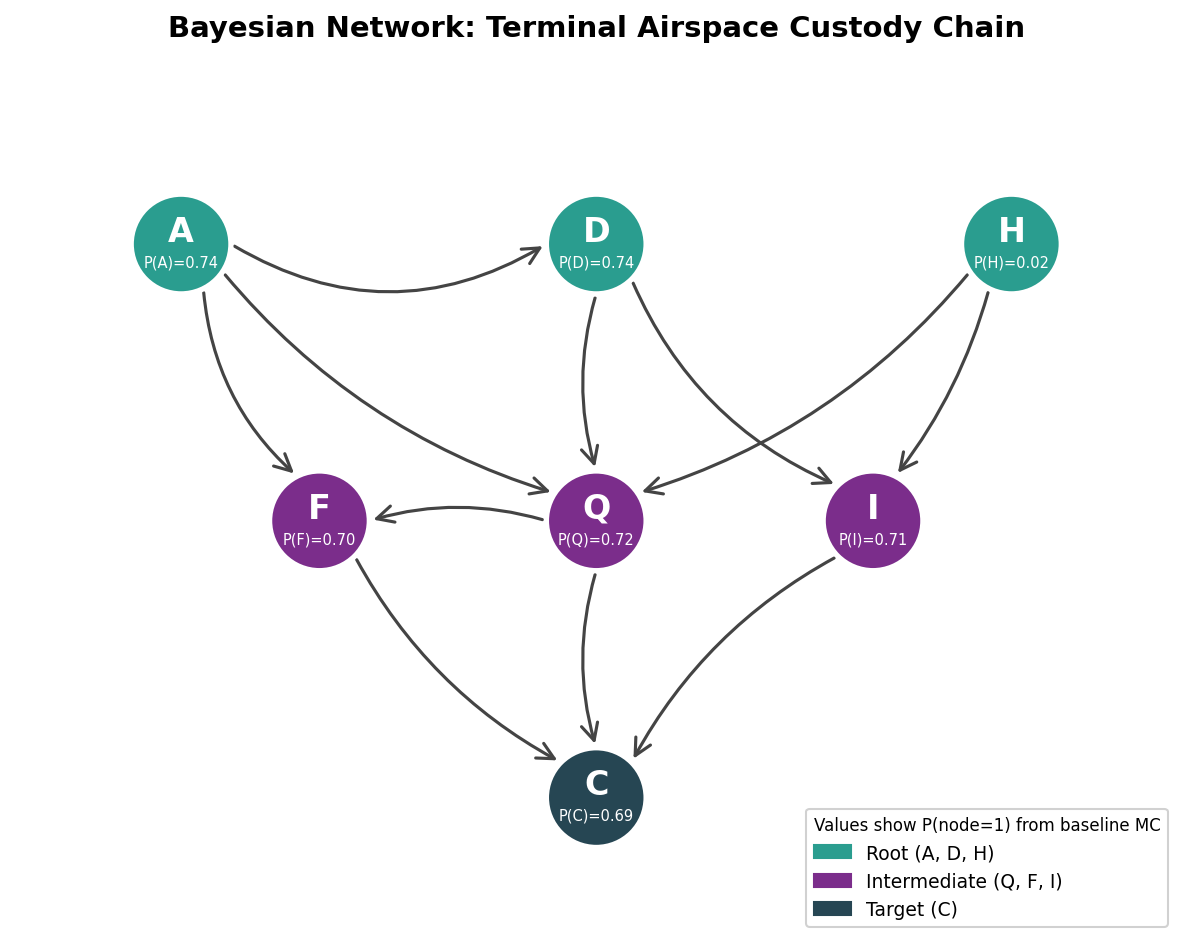
\includegraphics[width=0.85\linewidth]{figures/bn_structure.png}
    \caption{Seven-node BN DAG over the custody chain with marginal probabilities from baseline Monte Carlo estimation. Node shading indicates marginal $P(X{=}1)$.}
    \label{fig:bn_structure}
\end{figure}

\subsection{Failure Mode Vulnerability Ranking}
\label{sec:vulnerability}

Table~\ref{tab:vulnerability} reports the vulnerability delta $\Delta_i$ for each of the six upstream BN nodes under the do-calculus intervention $\mathrm{do}(X_i = 0)$. Fusion continuity ($F$) is the highest-vulnerability node with $\Delta_F = +0.985$, meaning that forcing fusion continuity to fail eliminates nearly all custody probability. This result is physically interpretable: because custody is defined as $C = A \wedge Q \wedge F$, any persistent failure in $F$ directly prevents custody regardless of the state of other nodes. Precision tracking ($Q$) and identity persistence ($I$) are the second and third most vulnerable nodes, reflecting their role as necessary precursors to fusion continuity. Availability ($A$) and detection ($D$) rank fourth and fifth with identical deltas, indicating that at the ADS-B detection probability of 0.99, detection failures are rare and availability is the binding constraint.

The most operationally significant finding is the negative delta for handoff ($H$): $\Delta_H = -0.340$. This indicates that forcing handoffs to fail, that is, eliminating ownership transfers entirely, actually reduces custody. The physical explanation is that in a dynamic multi-satellite constellation, handoffs are not custody interruptions but custody enablers: they transfer ownership to the best-positioned satellite before the current owner loses line-of-sight. Preventing handoffs causes satellites to retain ownership beyond their effective coverage window, producing custody gaps that would otherwise be filled by a successor satellite. This finding contrasts with the intuitive assumption that handoffs are a vulnerability, and has direct implications for the mitigation analysis in Section~\ref{sec:mitigations}. It also differs qualitatively from the kill chain analysis in~\cite{Saeed2025DOEFramework}, where detection was the dominant failure mode; in the custody chain, internal continuity constraints dominate over external detection probability.

\begin{table}[h]
    \caption{BN vulnerability ranking by do-calculus intervention $\mathrm{do}(X_i{=}0)$. Positive delta indicates custody loss when node fails; negative delta indicates custody improves when node fails.}
    \label{tab:vulnerability}
    \centering
    \begin{tabular}{clcc}
        \toprule
            Rank & Node & $\Delta_i$ & Interpretation \\
        \midrule
            1 & $F$ (Fusion continuity) & $+0.985$ & Highest-impact failure \\
            2 & $Q$ (Precision tracking) & $+0.952$ & Precursor to $F$ \\
            3 & $I$ (Identity persistence) & $+0.940$ & Identity chain failure \\
            4 & $A$ (Availability) & $+0.927$ & Binding availability constraint \\
            5 & $D$ (Detection) & $+0.927$ & Rarely fails at $p{=}0.99$ \\
            6 & $H$ (Handoff) & $-0.340$ & Handoffs enable custody \\
        \bottomrule
    \end{tabular}
\end{table}

\begin{figure}[h]
    \centering
    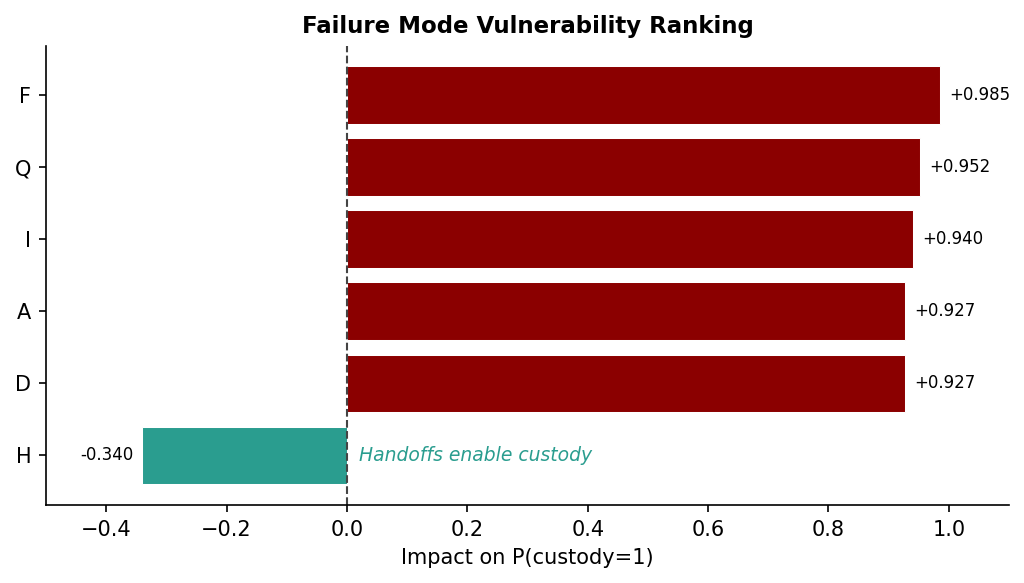
\includegraphics[width=0.85\linewidth]{figures/failure_modes.png}
    \caption{BN vulnerability ranking: do-calculus delta $\Delta_i$ for each custody chain node under $\mathrm{do}(X_i{=}0)$ intervention. Positive values indicate custody loss; negative values indicate custody improves when the node is forced to fail.}
    \label{fig:failure_modes}
\end{figure}

\subsection{Mitigation Analysis}
\label{sec:mitigations}

Table~\ref{tab:mitigation} reports the mitigation delta for four interventions applied via $\mathrm{do}(X_i{=}1)$. Perfect availability, eliminating all satellite coverage gaps, produces the largest custody improvement of $+0.239$ ($+34.5\%$), confirming that constellation geometry and orbital coverage are the primary operational levers. Perfect detection produces a much smaller improvement of $+0.064$ ($+9.2\%$), reflecting the already high ADS-B detection probability. Eliminating handoffs entirely yields a negligible improvement of $+0.006$ ($+0.8\%$), consistent with the finding that handoffs are enablers rather than vulnerabilities. Most significantly, implementing hysteresis, a strategy that reduces handoff frequency by requiring a sustained proximity advantage before transferring ownership, produces a custody decrease of $-0.096$ ($-13.9\%$). This counter-intuitive result occurs because hysteresis prevents timely ownership transfers to better-positioned satellites, causing the current owner to retain custody beyond its effective coverage window and producing the same gap-filling failure described in the handoff analysis above.

\begin{table}[h]
    \caption{Mitigation analysis via $\mathrm{do}(X_i{=}1)$ interventions. Baseline $P(C{=}1) = 0.693$.}
    \label{tab:mitigation}
    \centering
    \begin{tabular}{lccc}
        \toprule
            Mitigation & $\Delta P(C{=}1)$ & Improvement & Mechanism \\
        \midrule
        Perfect availability & $+0.239$ & $+34.5\%$ & Eliminates coverage gaps \\
        Perfect detection & $+0.064$ & $+9.2\%$ & Marginal at $p{=}0.99$ \\
        Eliminate handoffs & $+0.006$ & $+0.8\%$ & Negligible --- handoffs help \\
        Hysteresis (reduce $H$) & $-0.096$ & $-13.9\%$ & Blocks timely transfers \\
        \bottomrule
    \end{tabular}
\end{table}

\begin{figure}[h]
    \centering
    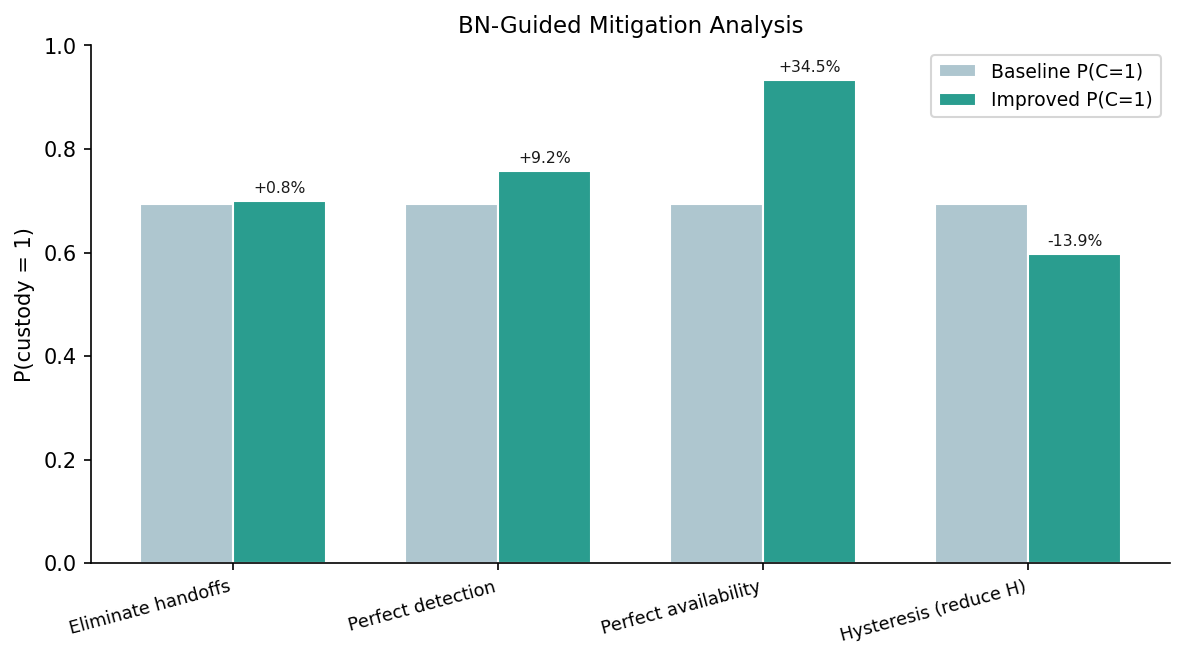
\includegraphics[width=0.85\linewidth]{figures/mitigations.png}
    \caption{Mitigation analysis: custody probability change under $\mathrm{do}(X_i{=}1)$ interventions. Baseline $P(C{=}1) = 0.693$ shown as dashed reference line.}
    \label{fig:mitigations}
\end{figure}

\subsection{DoE Factor Analysis}
\label{sec:doe_analysis}

Table~\ref{tab:doe} reports the Random Forest feature importance scores from the 270-run DoE. Sensor type accounts for 99.9\% of the variance in custody rate across all configurations, dwarfing the contributions of constellation size, target count, and simulation duration, which are collectively responsible for less than 0.1\% of the variance. This result is consistent with the main effects analysis shown in Figure~\ref{fig:doe_main}: ADS-B configurations produce custody rates in the range [0.65, 0.77], MLAT configurations produce rates in [0.39, 0.43], and Mode-S configurations produce a custody rate of approximately zero across all constellation sizes and target counts.

The Mode-S structural failure is a direct consequence of the interaction between sensor update rate and simulation tick rate. Mode-S interrogation updates every 4~seconds, but the simulation tick is $dt = 2$~s. The BN custody definition requires $Q \geq 3$ consecutive detections and $F \geq 3$ consecutive $Q{=}1$ ticks. Because Mode-S produces a detection at most every other tick, the consecutive detection counter can never reach three before resetting, a structural impossibility independent of detection probability, constellation geometry, or target count. This finding identifies sensor update rate relative to the tracking loop tick rate as an architectural constraint, not merely a performance parameter. Any sensor with an update interval slower than the simulation tick rate is structurally incompatible with custody definitions that require consecutive detections, regardless of all other system parameters. This extends the DoE methodology of~\cite{Saeed2025DOEFramework} by revealing a categorical rather than continuous factor effect, a qualitative failure mode that cannot be interpolated from performance data alone.

\begin{table}[h]
    \caption{Random Forest feature importance scores from 270-run DoE (54 configs $\times$ 5 seeds). Scores sum to 1.0.}
    \label{tab:doe}
    \centering
    \begin{tabular}{lcc}
    \toprule
        Factor & Levels & Importance \\
    \midrule
    Sensor type & ADS-B, Mode-S, MLAT & 0.999 \\
    Number of satellites & 8, 12, 16 & 0.000 \\
    Number of targets & 10, 20, 30 & 0.000 \\
    Simulation duration (s) & 3600, 7200 & 0.000 \\
    \bottomrule
    \end{tabular}
\end{table}

\begin{figure}[h]
    \centering
    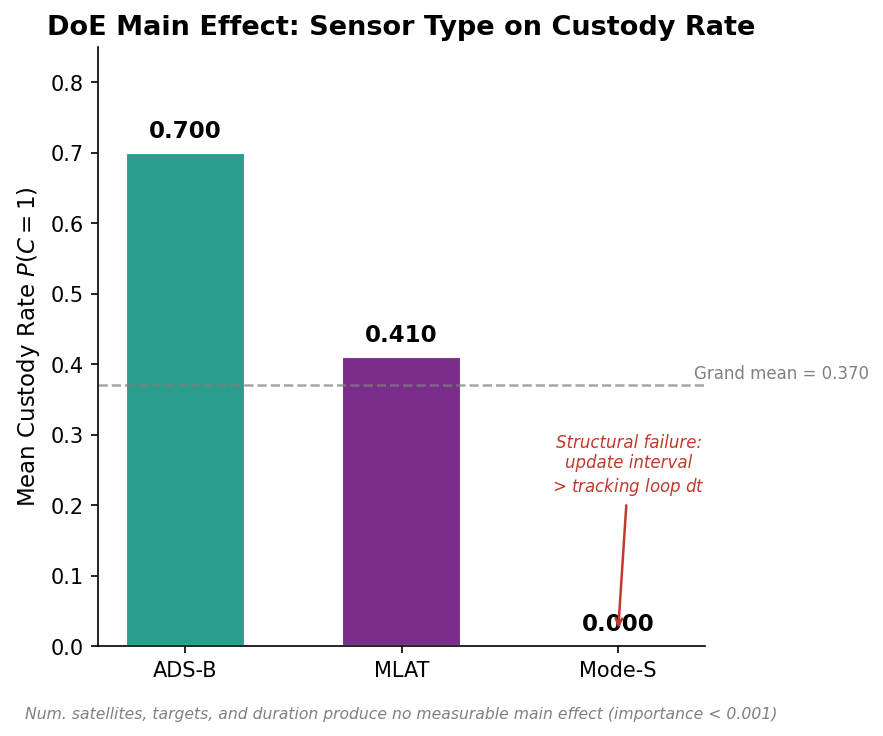
\includegraphics[width=0.85\linewidth]{figures/doe_main_effects.png}
    \caption{DoE main effect of sensor type on mean custody rate $P(C{=}1)$ across 270 simulation runs (54 configurations $\times$ 5 seeds). Mode-S produces zero custody due to the architectural constraint of Eq.~\ref{eq:constraint}. Number of satellites, targets, and simulation duration produce no measurable main effect (Random Forest importance $< 0.001$).}
    \label{fig:doe_main}
\end{figure}

\subsection{Sensitivity Analysis}
\label{sec:sensitivity}

The DoE results establish sensor type as the dominant architectural factor, but do not reveal the shape of the custody response to sensor parameters within each modality. Two parametric sweeps were conducted to characterize this sensitivity.

Figure~\ref{fig:update_sweep} shows custody rate as a function of sensor update interval from 1 to 10 seconds, with all other parameters held at baseline. Custody remains at the baseline level of 0.705 for update intervals $\leq dt = 2$~s, then collapses to zero at update intervals $> dt$. The transition is a step discontinuity, not a gradual degradation: any sensor updating slower than the tracking loop tick rate cannot sustain the consecutive detection counters required for $Q$ and $F$, regardless of its detection 
probability. This establishes a necessary condition for custody compatibility:

\begin{equation}
    \tau_{\mathrm{sensor}} \leq dt
    \label{eq:constraint}
\end{equation}

where $\tau_{\mathrm{sensor}}$ is the sensor update interval and $dt$ is the tracking loop tick rate. Sensors violating Eq.~\ref{eq:constraint} produce 
zero custody independent of all other system parameters.

\begin{figure}[h]
    \centering
    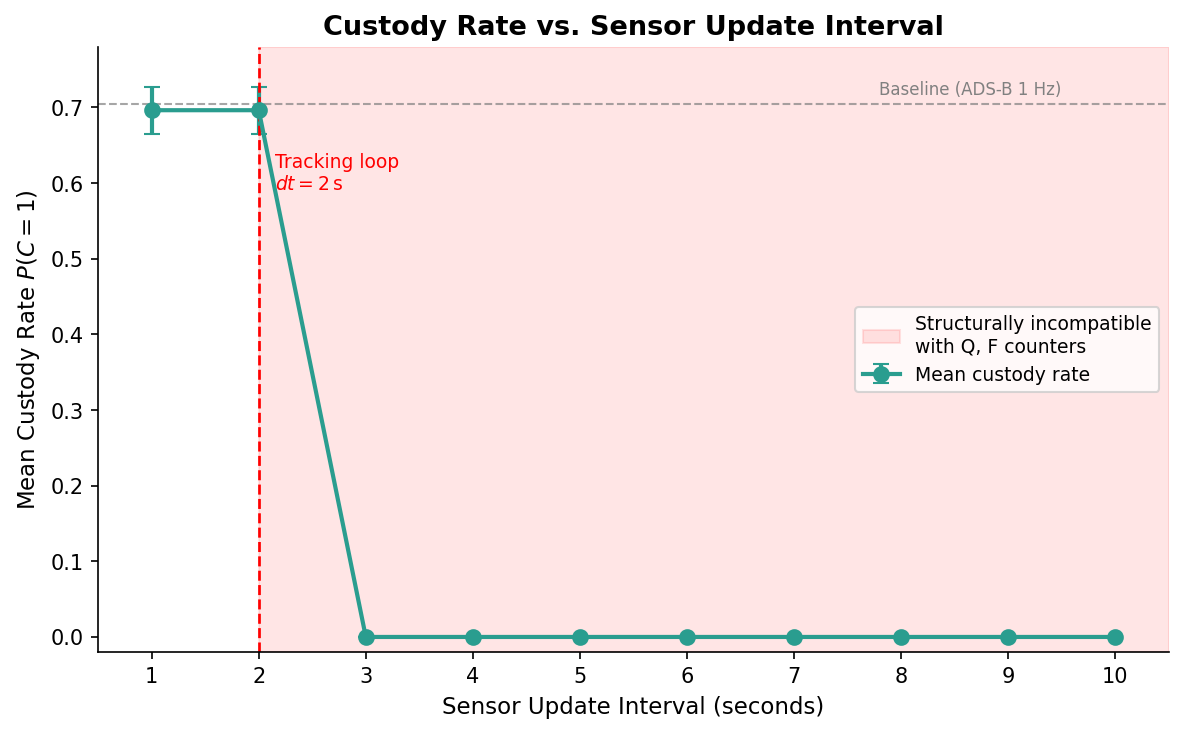
\includegraphics[width=0.9\linewidth]
        {figures/sensor_update_sweep.png}
    \caption{Custody rate vs.\ sensor update interval 
        (10 seeds per point, baseline configuration: 16 satellites, 20 targets, 7200~s). Custody remains at the ADS-B baseline of 0.705 for update intervals $\leq dt = 2$~s (red dashed line), then collapses to zero for all intervals $> dt$. The step discontinuity establishes a necessary compatibility condition, Eq.~\ref{eq:constraint}, independent of detection probability or constellation geometry. Shaded region indicates structural incompatibility with the $Q$ and $F$ consecutive detection counters.}
    \label{fig:update_sweep}
\end{figure}

Figure~\ref{fig:det_sweep} shows custody rate as a function of detection probability $p_{\mathrm{det}}$ for ADS-B (1~Hz) and MLAT (2~Hz), both satisfying Eq.~\ref{eq:constraint}. Custody is strongly sensitive to $p_{\mathrm{det}}$ across the full range $[0.50, 0.99]$, increasing from near zero at $p_{\mathrm{det}} = 0.50$ to the baseline operating values at $p_{\mathrm{det}} = 0.99$ (ADS-B) and $p_{\mathrm{det}} = 0.90$ (MLAT). Crucially, ADS-B and MLAT produce nearly identical custody curves despite different update rates, indicating that once Eq.~\ref{eq:constraint} is satisfied, detection probability becomes the primary determinant of custody within a sensor modality. The BN mitigation result $\Gamma_D = +0.064$ reported in Table~\ref{tab:mitigation} reflects the flat slope of the curve near $p_{\mathrm{det}} = 0.99$; at lower operating points the marginal benefit of improving detection probability is considerably larger.

\begin{figure}[h]
\centering
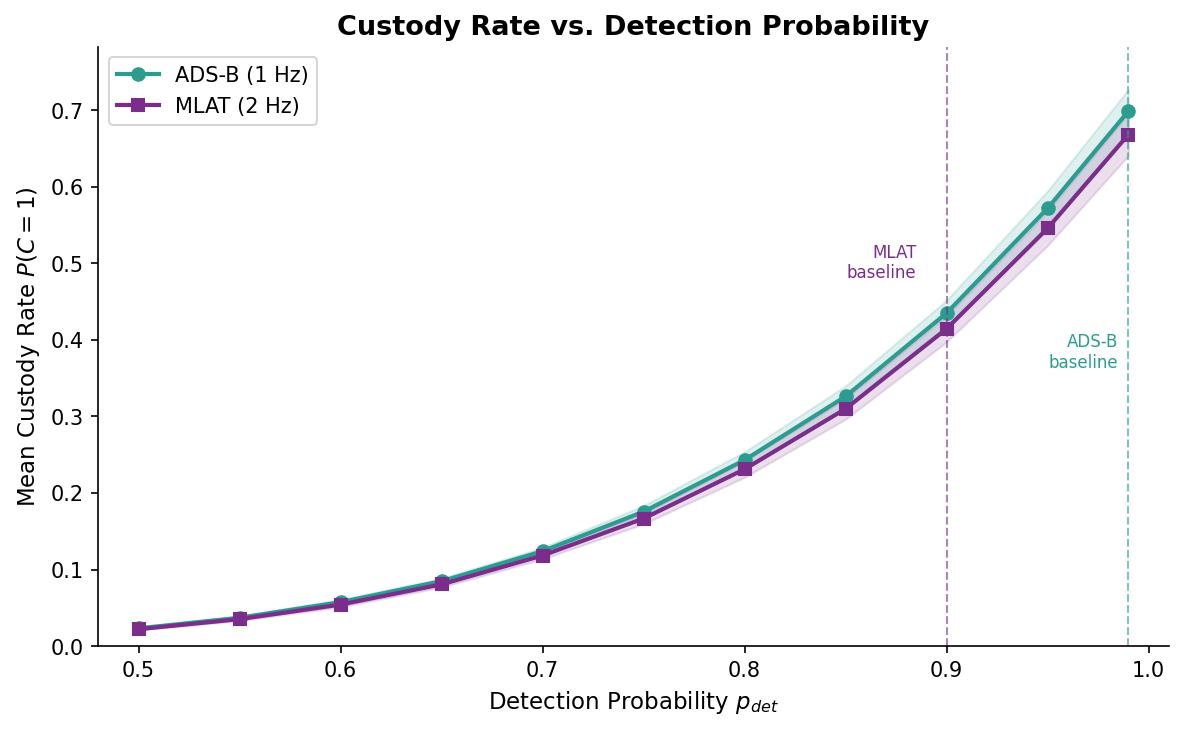
\includegraphics[width=0.9\linewidth]
    {figures/detection_prob_sweep.png}
    \caption{Custody rate vs.\ detection probability $p_{\mathrm{det}}$ for ADS-B (1~Hz, teal) and MLAT (2~Hz, purple), both satisfying the update rate constraint of Eq.~\ref{eq:constraint}. Shaded bands show $\pm 1$ standard deviation across 10 seeds per point. ADS-B and MLAT produce near-identical custody sensitivity curves despite different update rates, confirming that detection probability governs custody within a compatible modality. The BN mitigation delta $\Gamma_D = +0.064$ corresponds to the shallow slope near the ADS-B operating point of $p_{\mathrm{det}} = 0.99$.}
    \label{fig:det_sweep}
\end{figure}

This sensitivity analysis has two direct operational implications. First, the update rate constraint of Eq.~\ref{eq:constraint} is a hard architectural boundary: system designers must verify sensor update compatibility with the tracking loop before any performance analysis is meaningful. Second, in degraded environments where ADS-B detection probability falls below 0.90, due to equipage gaps, RF interference, or deliberate jamming, MLAT provides comparable custody performance at the same $p_{\mathrm{det}}$, making it a viable fallback modality provided its update rate satisfies Eq.~\ref{eq:constraint}. Together, Figures~\ref{fig:update_sweep} and~\ref{fig:det_sweep} 
characterize the two-dimensional sensor design space: update rate determines structural compatibility, and detection probability determines custody performance within the compatible region.

% ======================================================================
% 5. CONCLUSION AND FUTURE WORK
% ======================================================================
\section{Conclusion and Future Work}
\label{sec:conclusion}

This paper presented a Bayesian Network guided vulnerability analysis of aircraft custody in terminal airspace, extending the GoDSAT framework~\cite{Saeed2026GoDSATRL} with the DoE-BN methodology established in~\cite{Saeed2025DOEFramework,Saeed2025BNDOE}. A Python reimplementation of the GoDSAT 16-satellite CONUS constellation enabled 320 simulation runs across three sensor modalities and a full-factorial DoE. A seven-node BN over the custody chain, availability, detection, handoff, precision tracking, fusion continuity, identity persistence, and custody, was estimated from simulation data and analyzed via do-calculus interventions. The baseline custody rate of 0.705 (95\% CI $[0.697, 0.712]$) is consistent with the results of ~\cite{Saeed2026GoDSATRL}, validating the reimplementation.

Three findings stand out. First, fusion continuity ($F$) is the dominant custody vulnerability ($\Delta_F = +0.985$), not detection ($\Delta_D = +0.927$) as in the kill chain analysis of~\cite{Saeed2025DOEFramework}. This confirms that custody and survivability chains have qualitatively different failure structures, and that the dominant node depends on the chain's internal continuity requirements rather than its detection sensitivity alone. Second, handoffs are custody enablers, not vulnerabilities: preventing them reduces custody by 13.9\%, because they allow the constellation to pass ownership to better-positioned satellites before coverage gaps open. Third, sensor update rate is an architectural constraint: Mode-S at a 4-second interval is structurally incompatible with a 2-second tracking loop that requires consecutive detections, producing zero custody regardless of all other factors. Sensor type accounts for 99.9\% of custody variance in the DoE, a categorical dominance that cannot be recovered by increasing constellation size or extending simulation duration.

Future work will extend this analysis in four directions. First, replacing the Bernoulli sensor model with an EKF/UKF tracker and interacting multiple model (IMM) fusion will introduce realistic track uncertainty and association ambiguity, enabling BN CPTs to be estimated from track quality metrics rather than binary detection flags. Second, integration with live ADS-B data from the OpenSky network~\cite{opensky} will allow CPTs to be validated against real terminal airspace operations. Third, the do-calculus framework will be extended to support multi-node joint interventions, enabling analysis of interaction effects between mitigations, for example, whether combining perfect availability with ADS-B selection produces super-additive custody improvement. Fourth, the BN framework developed here is directly extensible to the multi-sensor GoDSAT-AT architecture, which fuses ADS-B, MLAT, and LEO EO/IR sources through an IMM-EKF/UKF core. Estimating joint CPTs across heterogeneous sensor modalities will require extending the current seven-node single-sensor BN to a multi-layer network where sensor-level nodes feed into track-level fusion nodes, enabling vulnerability analysis at the fusion layer rather than the detection layer alone. The do-calculus framework and Laplace-smoothed CPT estimation developed in this paper transfer directly to this extended topology, providing a principled foundation for multi-sensor custody vulnerability analysis in future work.

% ======================================================================
% APPENDIX
% ======================================================================
\appendix

\section{BN NODE DEFINITIONS AND SIMULATION PARAMETERS}
\label{sec:appendix}

\subsection{BN Node Definitions}

The seven BN nodes are derived directly from GoDSAT-AT simulation signals. Table~\ref{tab:nodes} provides formal definitions for each node as implemented in the Python simulation.

\begin{table}[h]
\caption{BN node definitions. All nodes are binary (0/1) at each simulation tick.}
\label{tab:nodes}
\centering
\begin{tabular}{cll}
\toprule
Node & Name & Definition \\
\midrule
$A$ & Availability & Satellite live AND target detected this tick \\
$D$ & Detection & Target within satellite FOV half-cone \\
$H$ & Handoff & ClaimMap ownership changed since previous tick \\
$Q$ & Precision tracking & $\geq 3$ consecutive $D{=}1$ ticks \\
$F$ & Fusion continuity & $\geq 3$ consecutive $Q{=}1$ ticks \\
$I$ & Identity persistence & Continuously tracked $\geq 10$~s \\
$C$ & Custody & $A \wedge Q \wedge F$ \\
\bottomrule
\end{tabular}
\end{table}

\subsection{Simulation Parameters}

Table~\ref{tab:params} summarizes the simulation parameters used in all baseline and DoE runs. Constellation orbital elements match those defined in~\cite{Saeed2026GoDSATRL}.

\begin{table}[h]
\caption{Simulation parameters for baseline and DoE runs.}
\label{tab:params}
\centering
\begin{tabular}{lll}
\toprule
Parameter & Value & Description \\
\midrule
$dt$ & 2~s & Simulation timestep \\
Constellation & 16 satellites & Two planes, RAAN $50^\circ$/$120^\circ$ \\
Semi-major axis & 2000~km & Per~\cite{Saeed2026GoDSATRL} \\
Eccentricity & 0.1 & Per~\cite{Saeed2026GoDSATRL} \\
Inclination & $90^\circ$ & Per~\cite{Saeed2026GoDSATRL} \\
Targets (baseline) & 20 & CONUS great-circle arcs \\
Duration (baseline) & 7200~s & Two-hour simulation window \\
MC runs (baseline) & 50 & Independent random seeds \\
DoE configurations & 54 & Full factorial $3 \times 3 \times 3 \times 2$ \\
DoE seeds per config & 5 & Total 270 simulation runs \\
ADS-B update rate & 1~Hz & $p_{\mathrm{det}} = 0.99$~\cite{adsb_faa} \\
Mode-S update rate & 0.25~Hz & $p_{\mathrm{det}} = 0.95$ \\
MLAT update rate & 0.5~Hz & $p_{\mathrm{det}} = 0.90$~\cite{opensky} \\
\bottomrule
\end{tabular}
\end{table}

% ======================================================================
% ACKNOWLEDGMENTS
% ======================================================================
\acknowledgments

The authors gratefully acknowledge the Computer and Information Technology (CIT) program within the Johns Hopkins University Whiting School of Engineering, Engineering for Professionals, which encompasses Artificial Intelligence, Computer Science, Cybersecurity, Data Analytics, Data Science, and Information Systems Engineering. The support provided through this program was instrumental to this work.

% ======================================================================
% REFERENCES
% ======================================================================
\bibliography{bibliographies}
\bibliographystyle{spiebib}

\end{document}


% \documentclass[]{spie}  %>>> use for US letter paper
% %\documentclass[a4paper]{spie}  %>>> use this instead for A4 paper
% %\documentclass[nocompress]{spie}  %>>> to avoid compression of citations

% \renewcommand{\baselinestretch}{1.0} % Change to 1.65 for double spacing

% \usepackage{algorithm}
% \usepackage{algpseudocode}

% \usepackage{pgf}
% \usepackage{tikz}
% \usetikzlibrary{intersections}
% \usetikzlibrary{arrows.meta,calc,positioning,fit,shapes.misc}
% \usetikzlibrary{backgrounds,shapes.geometric,math}

% \usepackage{pgfplots}
 
% \usepackage{amsmath,amsfonts,amssymb}
% \usepackage{graphicx}
% \usepackage[colorlinks=true, allcolors=blue]{hyperref}

% \title{Bayesian Network Guided Vulnerability Analysis of Detection, Fusion Continuity, and Sensor Handoffs for Aircraft Custody in Terminal Airspace}

% \author[a]{Amir K. Saeed}
% \author[a]{Alhassan S. Yasin, PhD}
% \author[b]{Thomas C. Cheng}
% \author[a]{Benjamin A. Johnson}
% \author[a]{Erhan Guven, PhD}
% \author[a]{Benjamin M. Rodriguez, PhD}
% \affil[a]{ Whiting School of Engineering EP Program, Johns Hopkins University}
% \affil[a]{Johns Hopkins Applied Physics Laboratory}

% \authorinfo{Further author information: Send correspondence to thomas.cheng@jhuapl.edu}

% % Option to view page numbers
% \pagestyle{empty} % change to \pagestyle{plain} for page numbers   
% \setcounter{page}{301} % Set start page numbering at e.g. 301
 
% \begin{document} 
% \maketitle

% % =======================
% % Short Abstract (≈150–180 words)
% % =======================
% \begin{abstract}
% We present a Bayesian Network (BN) guided method to identify and mitigate vulnerabilities in aircraft custody within terminal airspace, focusing on detection, fusion continuity, and sensor handoffs. Built on GoDSAT-AT, heterogeneous space–air–ground sources for Automatic Dependent Surveillance-Broadcast (ADS-B), Mode-S, multilateration (MLAT), low Earth orbit (LEO) electro-optical/infrared (EO/IR), synthetic aperture radar (SAR), airport surface radar, and tower EO, are fused with an IMM–EKF/UKF core to maintain identity-aware, uncertainty-quantified tracks. Reinforcement learning (RL) assigns sensing via a time-expanded ClaimMap and a cost-based ownership policy. From DataOps artifacts (ingest→validate→fuse→task→report), we estimate BN conditional probabilities for availability, detection, handoff realization, fusion continuity, identity persistence, and custody. BN forward/diagnostic inference ranks failure modes and quantifies “what-if” mitigations (priority lanes, hysteresis/cool-downs, SAR spotlights). In single-hub trials (20 flights/hour), BN guided changes increase custody by phase, reduce threshold and handoff latencies, and improve identity persistence with fewer false/duplicate tracks.
% \end{abstract}

% % =======================
% % Long Abstract (conference submission, < 5000 characters)
% % =======================
% \begin{abstract}
% This paper introduces a Bayesian Network (BN) guided vulnerability analysis for aircraft custody in terminal airspace that explains \emph{why} custody breaks and quantifies \emph{how} to fix it. Built atop the GoDSAT-AT environment, the pipeline ingests cooperative sources Automatic Dependent Surveillance–Broadcast (ADS-B), Mode-S, multilateration (MLAT), and non-cooperative modalities such as low Earth orbit (LEO) electro-optical/infrared (EO/IR), synthetic aperture radar (SAR), airport surface radar, and tower EO, under DataOps rigor (provenance, versioning, fitness-for-use diagnostics). An interacting multiple model extended/unscented Kalman filter (IMM EKF/UKF) with nearest-neighbor joint probabilistic data association (NNJPDA) style association and airport area of interest (AirportAOI) priors maintains identity-aware, uncertainty-quantified tracks through cooperative dropouts; optional fixed-lag smoothing supports productization.

% Sensor management is realized by reinforcement learning (RL) over a time-expanded ClaimMap function (latitude, longitude, altitude, and time) that reserves exclusive dwell windows and plans handoffs. A cost-based ownership rule generalizes proximity using look angle, predicted signal-to-noise ratio, slew/dwell, weather/occlusion, and mission priority; weights are tuned under centralized training with decentralized execution (CTDE). Imaging assets reuse GoDSAT’s Q-mode hill-climb centering; non-imagers honor reservations.

% We construct a BN whose nodes mirror logged events and key performance indicators (KPIs): availability, detection, Q-mode success, planned-handoff realization, fusion continuity, identity persistence, and custody. Conditional probability tables are estimated directly from GoDSAT-AT telemetry (validated measurements, innovations, ClaimMap reservations, handoff events), while design-of-experiments and surrogate modeling cover weather regimes (cloud decks/visibility), traffic intensity (push waves), sensor siting/sectors, and cost-weight sweeps. BN forward inference predicts custody shortfalls; diagnostic inference identifies dominant failure modes for observed losses; and sensitivity analysis quantifies the payoff of mitigations (e.g., hysteresis and cool-downs to stabilize handoffs, a high-priority sensing corridor along the final approach path, and SAR spotlighting under persistent cloud).

% In single-hub evaluations (20 flights/hour), ablations compare (i) proximity vs.\ costed ownership, (ii) ClaimMap on/off, and (iii) satellites-only vs.\ multi-sensor configurations. BN-guided adjustments yield higher custody by phase, reduced runway-threshold detection and handoff latencies, increased identity persistence, and fewer false/duplicate tracks. All stages emit signed, versioned artifacts (schemas, manifests, fusion posteriors, ClaimMap reservations, notebooks, LaTeX tables), enabling test and evaluation / verification and validation (T\&E/V\&V) and bit-for-bit re-runs. The result is a transparent, reproducible path from sensor fusion and RL tasking to decision-relevant risk reduction, centered on BN explanations of detection, fusion continuity, and handoff vulnerabilities.
% \end{abstract}

% % Include a list of keywords after the abstract 
% \keywords{Bayesian networks, multi-sensor fusion, aircraft custody, sensor handoffs, vulnerability analysis, evaluation, verification and validation,  risk reduction}






% %%%%%%%%%%%%%%%%%%%%%%%%%%%%%%%%%%%%%%%%%%%%%%%%%%%%%%%%%%%%%%%%%%%%%%%%%%%%%%
% \section{INTRODUCTION}
% \label{sec:intro}  % \label{} allows reference to this section
% %%%%%%%%%%%%%%%%%%%%%%%%%%%%%%%%%%%%%%%%%%%%%%%%%%%%%%%%%%%%%%%%%%%%%%%%%%%%%%


% %%%%%%%%%%%%%%%%%%%%%%%%%%%%%%%%%%%%%%%%%%%%%%%%%%%%%%%%%%%%%%%%%%%%%%%%%%%%%%
% \section{Related Work and Background}
% %%%%%%%%%%%%%%%%%%%%%%%%%%%%%%%%%%%%%%%%%%%%%%%%%%%%%%%%%%%%%%%%%%%%%%%%%%%%%%


% %%%%%%%%%%%%%%%%%%%%%%%%%%%%%%%%%%%%%%%%%%%%%%%%%%%%%%%%%%%%%%%%%%%%%%%%%%%%%%
% \section{Methodology}
% %%%%%%%%%%%%%%%%%%%%%%%%%%%%%%%%%%%%%%%%%%%%%%%%%%%%%%%%%%%%%%%%%%%%%%%%%%%%%%
% \label{sec:}


% %%%%%%%%%%%%%%%%%%%%%%%%%%%%%%%%%%%%%%%%%%%%%%%%%%%%%%%%%%%%%%%%%%%%%%%%%%%%%%
% \section{Analysis}
% \label{sec:sections}
% %%%%%%%%%%%%%%%%%%%%%%%%%%%%%%%%%%%%%%%%%%%%%%%%%%%%%%%%%%%%%%%%%%%%%%%%%%%%%%


% %%%%%%%%%%%%%%%%%%%%%%%%%%%%%%%%%%%%%%%%%%%%%%%%%%%%%%%%%%%%%%%%%%%%%%%%%%%%%%
% \section{Conclusion and Future Work}
% %%%%%%%%%%%%%%%%%%%%%%%%%%%%%%%%%%%%%%%%%%%%%%%%%%%%%%%%%%%%%%%%%%%%%%%%%%%%%%




% %%%%%%%%%%%%%%%%%%%%%%%%%%%%%%%%%%%%%%%%%%%%%%%%%%%%%%%%%%%%%%%%%%%%%%%%%%%%%%
% \appendix    %>>>> this command starts appendixes
% %%%%%%%%%%%%%%%%%%%%%%%%%%%%%%%%%%%%%%%%%%%%%%%%%%%%%%%%%%%%%%%%%%%%%%%%%%%%%%

% \section{MISCELLANEOUS}
% \label{sec:misc}



% \subsection{Equations}



% \subsection{Theorems}



% \acknowledgments % equivalent to \section*{ACKNOWLEDGMENTS}       
% Grateful acknowledgment to the program leadership at Whiting School of Engineering EP Program Johns Hopkins University for providing the opportunity to engage in research within aerospace and machine learning.

% % References
% \bibliography{report} % bibliography data in report.bib
% \bibliographystyle{spiebib} % makes bibtex use spiebib.bst

% \end{document} 
